\chapter{研究背景}
\label{chap:webapi}

 ユーザーの拡張現実や明晰夢における認識度や要求について事前調査、睡眠に関する調査、睡眠中に見たい夢の分析を行った。そしてDreamtravelerの開発に反映した点について述べる。

\section{拡張現実について調査}
人がどのような拡張現実を望んでいるかを調査するため、理系の学生7人、文系の学生7人、サラリーマン10人、主婦3人を含めた20〜60歳の男女27人にオンラインアンケートをした。これらのインタビュー結果を経て一般的なユーザのニーズを把握し、Dreamtravelerの有効性やDreamtravelerが解決すべき問題について明らかにする。

\subsection{拡張現実を体験するために一般的な人々が支払う金額}
各所公式ウェブサイトを掲載し、機能性やデザインの詳細を説明した上で、仮想現実を見る手段として次の選択肢から購入しようと思う商品を選んでもらった。

\begin{itemize}
\item OCULOUS Rift:85278円
\item ハコスコ:1500円
\item iWink:36478円
\item タカラトミー夢見工房:15984円
\item Dreamtraveler :無料
\end{itemize}

すると図\ref{userNeedCost}のように、一般ユーザーの中には拡張現実を体験するためにOCULOUS Riftなどの高額なデバイスを購入しようとする人は少ないということが分かった。1500円ハコスコだと少し数が増えるが、これらのデータから無料で簡単に手に入れることができるツールを多くの人が必要としていることが示唆された。

\begin{figure}[htbp]
\begin{center}
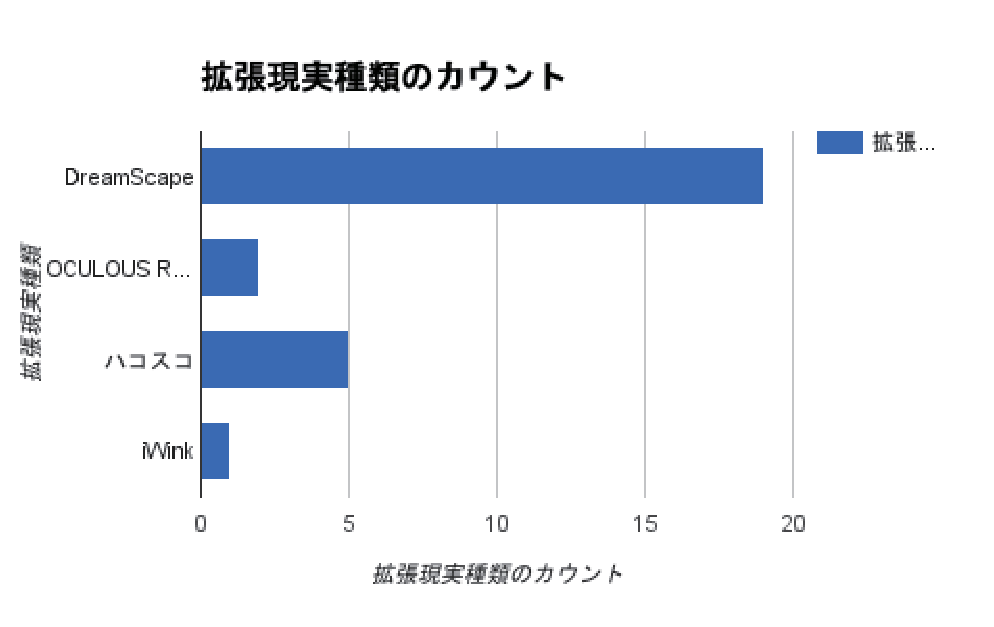
\includegraphics[width=15cm]{eps/VRselection.eps}
\caption{拡張現実を体験するために一般的ユーザーが選ぶデバイス}
 \label{userNeedCost}
\end{center}
\end{figure}

\subsection{拡張現実を体験したいタイミング }
拡張現実を体験したいタイミングとして、睡眠中と起きている時間帯でどちらが好ましいかについて調査を行った。すると睡眠中と答えたのは52\%、起床中と答えたのは48\%。このように結果にはあまり差がなかった。睡眠中を選択した人は理由として「睡眠時間の有効活用のため」と答えた。比べて起きている時と選択した人は「起きたら忘れてしまうかもしれないから、意識のある時に体験したい」と答えた。よってDreamTravelerの開発において、睡眠中の体験がユーザーにどのような印象を与えるかを研究することは意義があると考えられる。実際にユーザーがDreamTravelerを使用してどう感じたかに関しては後の第6章で述べる。

\section{睡眠に関する調査}
睡眠中に扱うアプリケーションの開発にあたって、睡眠自体を理解することは不可欠であ。事前調査によって明らかになった睡眠段階や夢についてここで記す。

\subsection{睡眠と睡眠段階(睡眠の深さのレベル)について}
 睡眠は身体を休めるためにある。そして人生の1/3を占める活動である。そして睡眠中人は2つの睡眠段階、REM睡眠とnonREM睡眠を90分間隔で行き来している\cite{Dement}。筑波大と理化学研究所の研究によるとREM睡眠中は記憶形成や脳機能回復の作用がある脳波(デルタ波)が多く見られるというのが通説である\cite{tsukuba}。そしてREM睡眠中は心拍数や眼球の運動が活発化する。REM睡眠の最中に起きたときは夢も比較的覚えているという研究もされている\cite{remNonRem}。一方nonREM睡眠中は脳も身体も休んでいる。\\
 図\ref{SleepHypnogram}は平均的な睡眠のサイクルを示したものである。睡眠に突入して初めてのREM睡眠は10〜12分でもっとも短い。2度目のREM睡眠は15〜20分。最後の夢は15分であるが、通常はアラームなどによって不意に中断されることが多い。平均的に一晩で5〜7回夢をみる。一般的な人生で人は6年間夢を見る。DreamTravelerはこの6年間をより充実感のある体験にするために貢献できるアプリケーションになる可能性があるのだ。

\begin{figure}[htbp]
\begin{center}
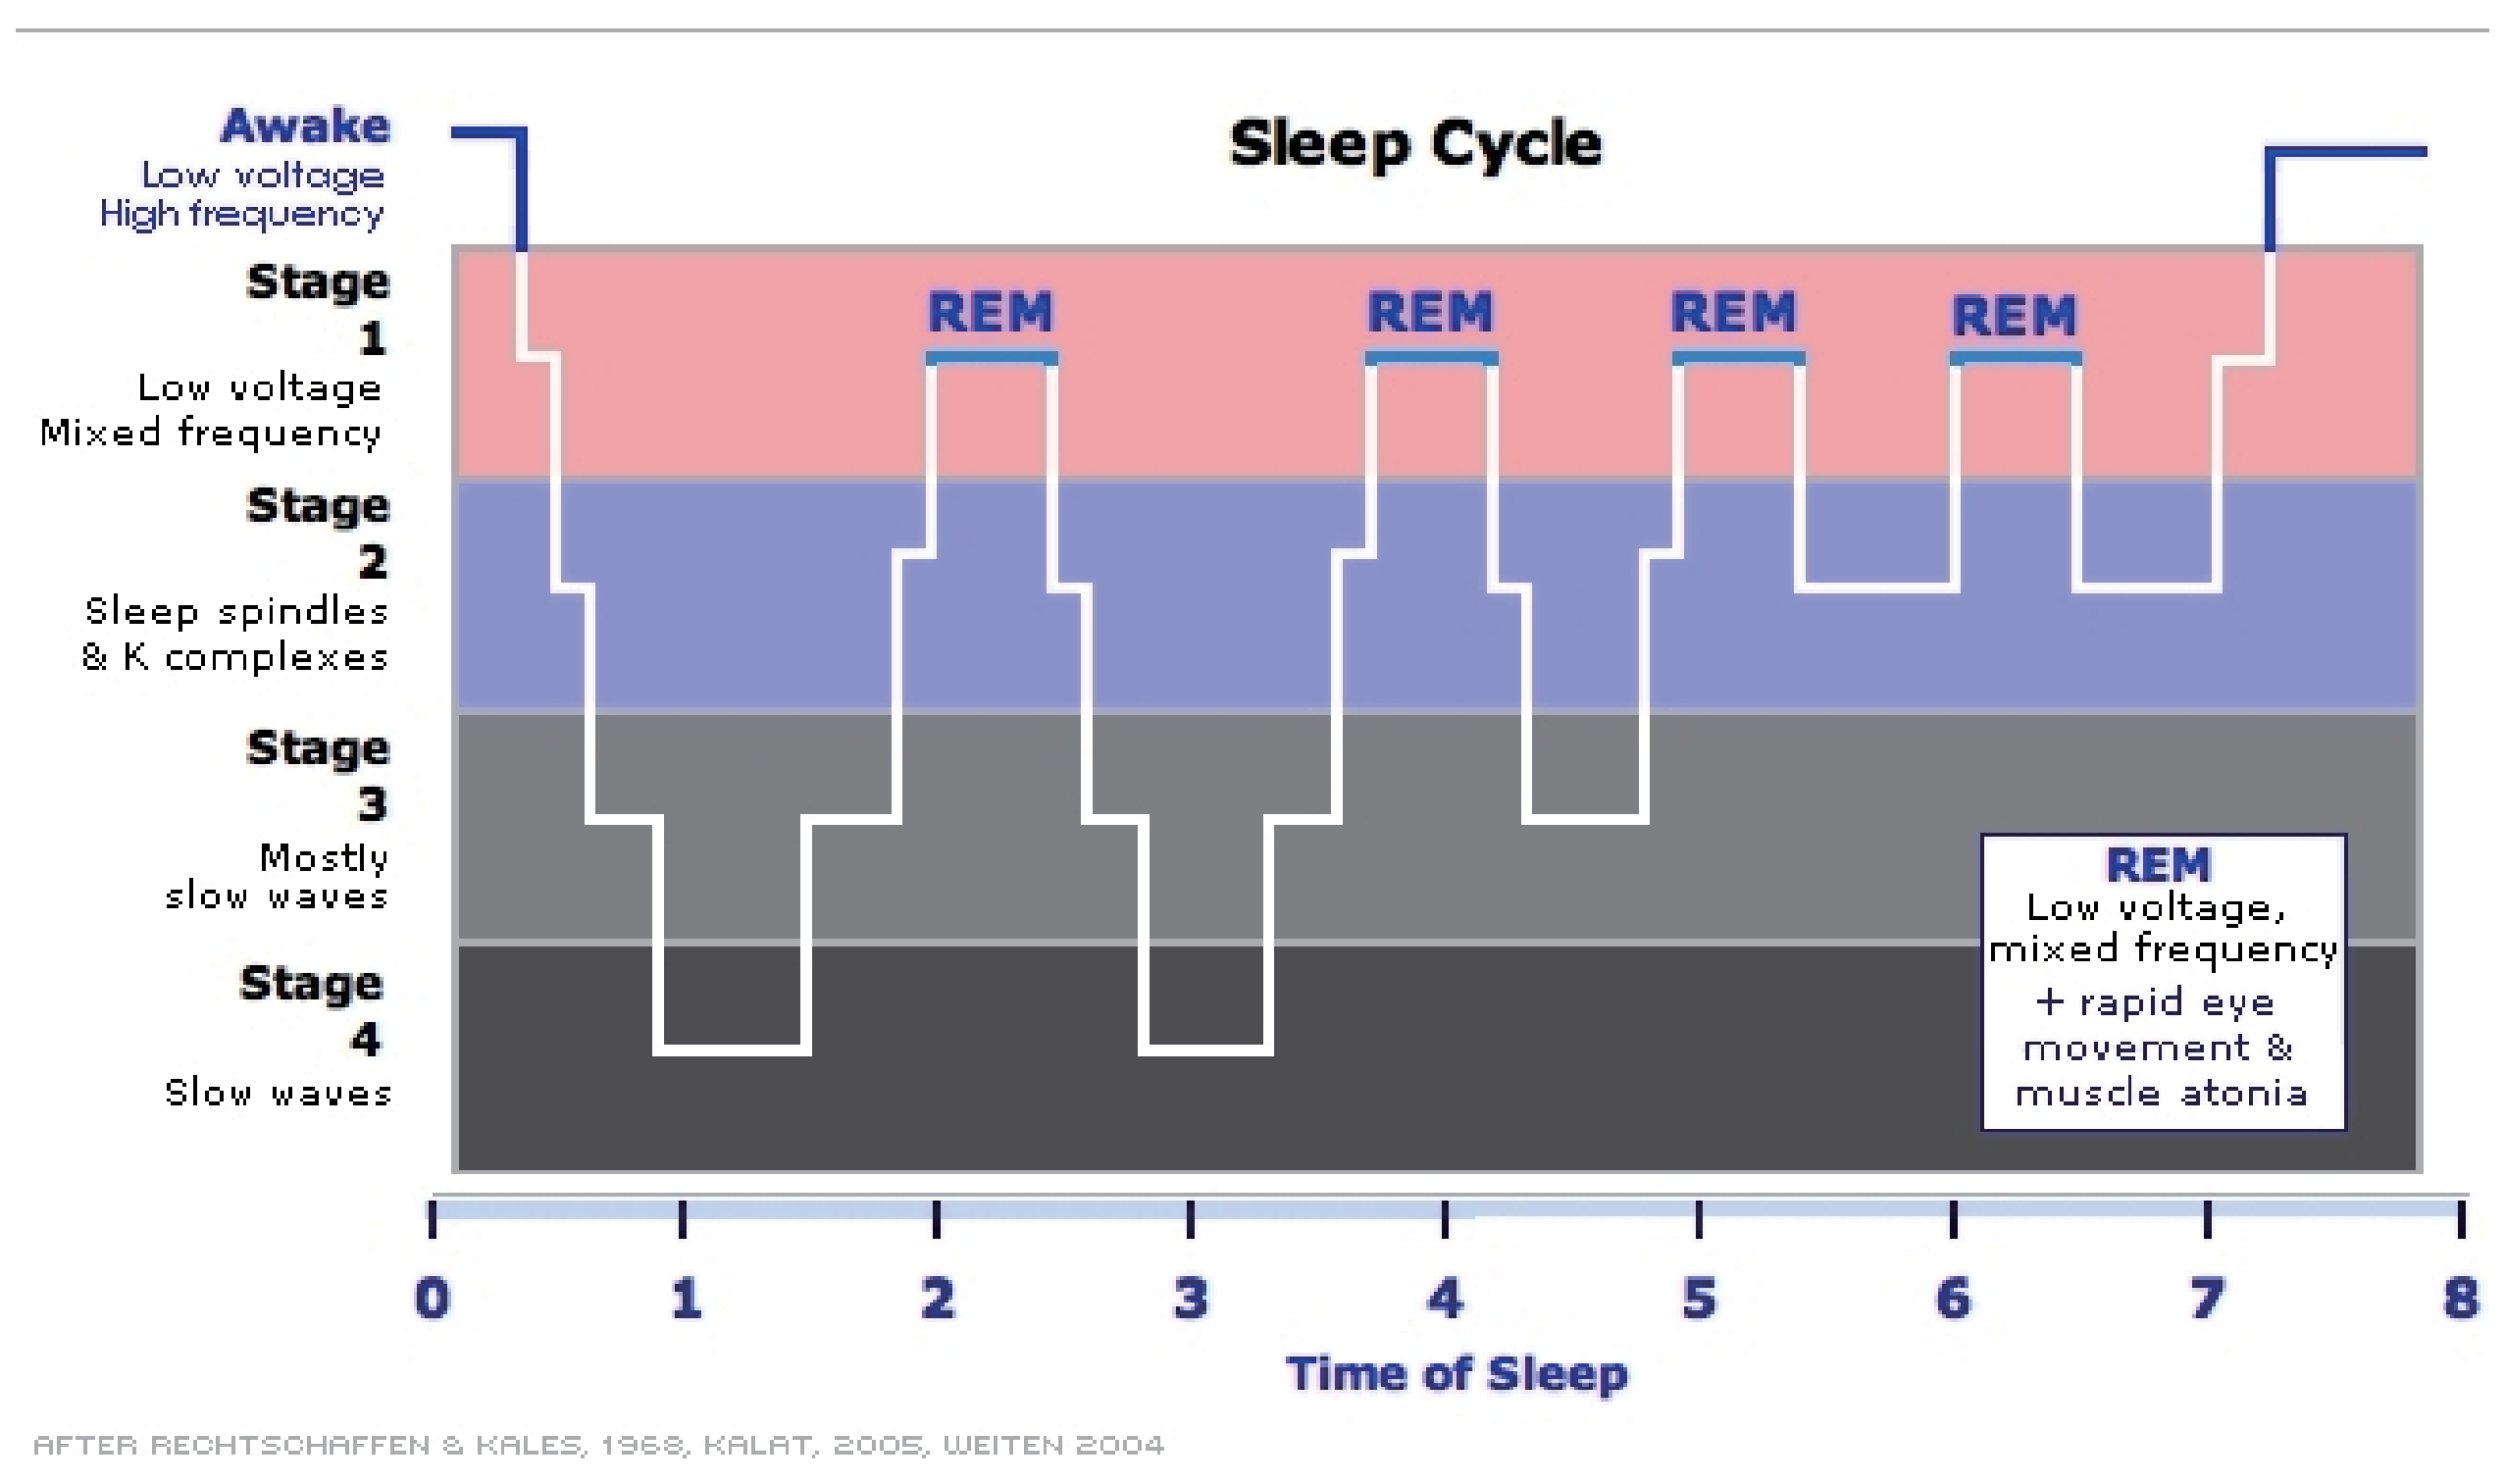
\includegraphics[width=15cm]{eps/SleepHypnogram.eps}
\caption{nonREMとREM睡眠}
\label{SleepHypnogram}
\end{center}
\end{figure}

\subsection{夢は現実であると錯覚するほどリアル}
 夢は空間、時間軸と、登場人物が非現実的な場合など不合理で異様な内容のことが多いが、大抵の場合人は、現実だと錯覚し夢を見ていることに気がつかない。それは論理的思考力を担う前頭前皮質の機能が低下しているためだ\cite{cortex}。起床後も夢での感情が現実で起きたかのように勘違いしてしまうほど、リアルな体験をした人も多いと推測される。起床後すぐに夢日記をとれば、本当の思い出のように夢の記憶が残る場合もある。

\subsection{人はなぜ夢を見るのか}
 心理学者であるSigmund Freudは1905年に無意識の欲求や感情、抑圧された子供の頃の記憶、整理的欲求などが夢に大きな影響を与えていると述べた\cite{freud}。一方で2006年にJie Zhangは夢は短期的な記憶を長期的な記憶に変換するためのプロセスであると述べている。この図\ref{brainZhang}は睡眠中の脳の働きを表す。脳の容量には限度があるため、睡眠中に過去の記憶の中で関連性の強い記憶を繋げたり、重複している内容や必要のない記憶を消しているのだ\cite{Zhang}。睡眠時間が減ると暗記能力が減るのもこれにより説明できる。
 幼児の平均睡眠時間は16時間でそのう内の50\%をREM睡眠が占める。一方成人の平均睡眠時間は7時間でREM睡眠も短いため、夢をあまり見なくなる。年齢が若いほどREM睡眠の周期が長いのは、経験すること全てが新しいため多くのことを記憶しなければならないことと、脳の空き容量が多いためと説明されている。

\begin{figure}[htbp]
\begin{center}
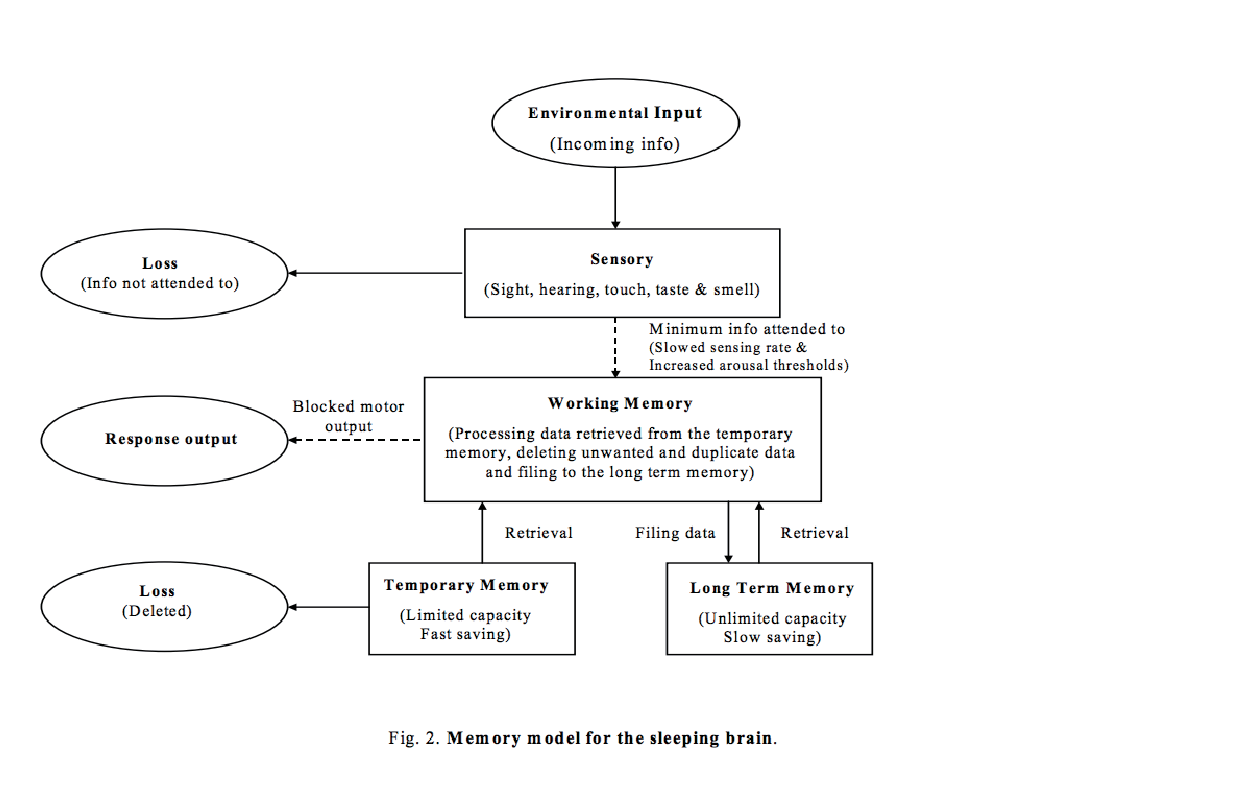
\includegraphics[width=15cm]{eps/sleepBrainModel.eps}
\caption{REM睡眠中の脳の働き睡眠}
\label{brainZhang}
\end{center}
\end{figure}

\subsection{睡眠段階のセンシング方法}
睡眠段階のセンシング方法として正確性が高いのは脳波センサーである。しかしそれ以外のセンシング方法もある。人はREM睡眠中に眼球が活発化し、心拍数が多少上がるので、眼球の運動と心拍によりセンシングが可能である。そして最後に体動だ。人は睡眠段階を移行させるために寝返りを行う習性があるとされている。要するに睡眠サイクルのスイッチのような働きをするのだ。\cite{negaeri}よって寝返りをモニタリングすれば睡眠段階をある程度センシングすることが可能であるということが通説である。

\section{明晰夢に関するアンケート調査}
\subsection{夢をどのくらい記憶しているか}
夢の操作に成功したとしてもその夢を覚えていなければ意味がない。そこで実験を始める前に一般的に人は夢の内容を起床後どのくらい覚えているのかをアンケート調査した。図\ref{rememberDream}がから読み取れるように、夢をよく覚えていると答えた人は少数だった。

\begin{figure}[htbp]
\begin{center}
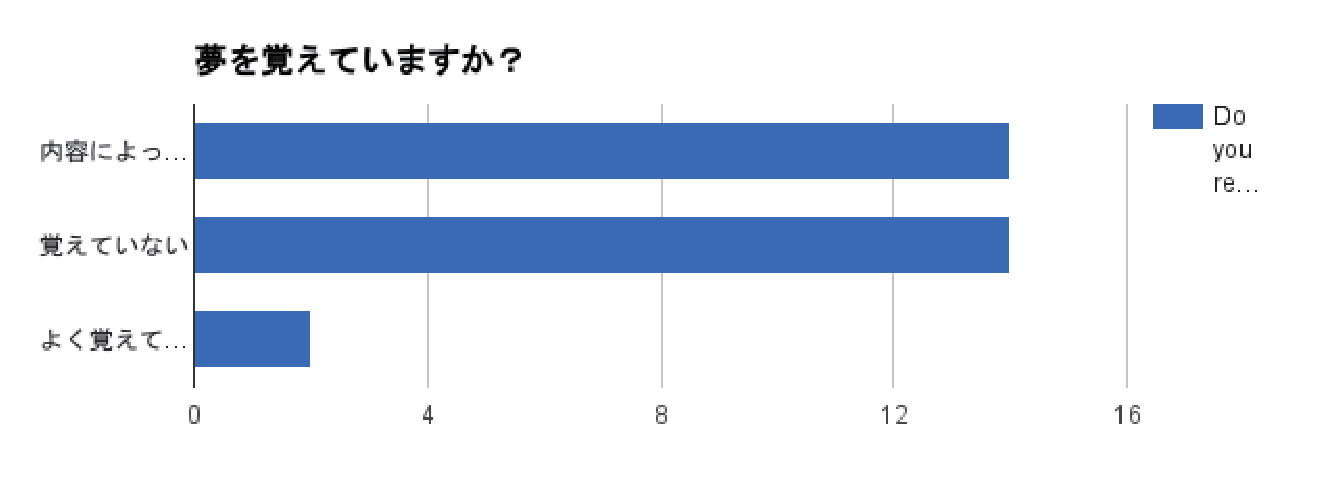
\includegraphics[width=15cm]{eps/remember.eps}
\caption{夢を覚えている比率}
\label{rememberDream}
\end{center}
\end{figure}

 覚えている夢は刺激的、怖い夢、繰り返し見た夢というのが多く、日常的な夢は忘れがちであるということが分かった。人は睡眠中の夢の90\%を起床後5分間で忘れるという。Jie ZhangによるとREM睡眠中は短期的な記憶を担っている脳は長期的な記憶への移行に注力していて、インプットの部分があまり機能していないためであると説明する。ただ起きてすぐに、夢日記で夢を記憶すれば覚えていられることが可能なのだ\cite{forgetDreams}。

\subsection{夢に影響を与えやすい外的刺激}
Sigmund Freudは「夢判断」の中で人は睡眠中の姿勢、環境、身体的刺激によって夢の内容が変化すると述べた\cite{freud}。睡眠中の人間の鼻先を羽毛でくすぐったときに、夢の内容に変化があったことを確認する実験を紹介している。そこで音、体制、匂い、振動、光、などの刺激の中で何が夢に一番影響を与えやすいのかのインタビューで調査をした。以下の図\ref{externalShigeki}がその結果を示す。音が他の刺激よりも影響を与えやすいということが分かった。また学術的にも聴覚と嗅覚は人間の生命維持を高めるために感度は低いが睡眠中も機能しているということが証明されている\cite{Zhang}。

\begin{figure}[htbp]
\begin{center}
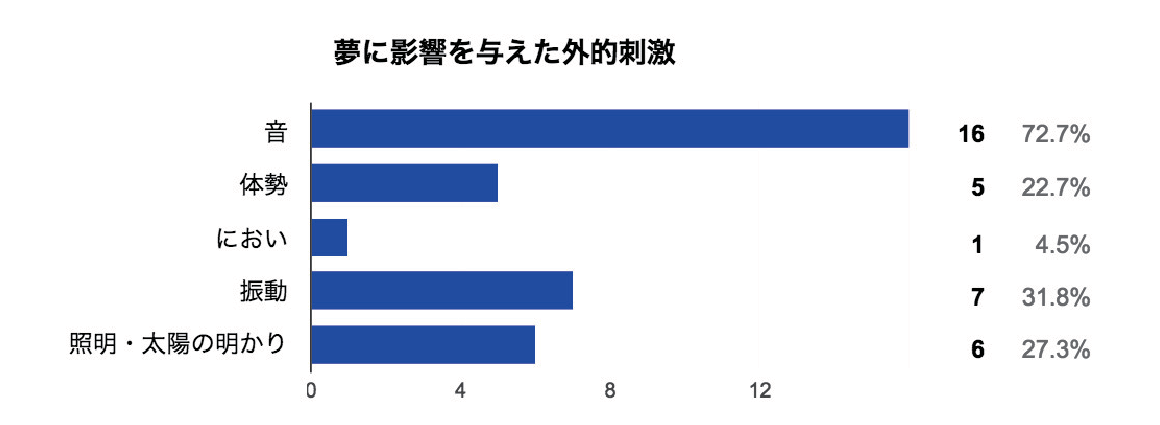
\includegraphics[width=15cm]{eps/input.eps}
\caption{夢に影響を与えた外的刺激}
\label{externalShigeki}
\end{center}
\end{figure}

\subsection{明晰夢のニーズ}
明晰夢を体験したいか否かで質問をしたところ77\%の人が体験したいと答えた。

\subsection{明晰夢で体験したい内容}
拡張現実で体験したい内容を調査結果から似ているものをカテゴリー別に分けて、図\ref{desiredDreamTpye}で示した。LOVEタイプ、癒しタイプ、元気欲しいタイプ、アドベンチャータイプ、ストーリータイプ、ビジネスタイプとあるがそれぞれの定義を述べる。LOVEタイプとは恋愛や性的行為などが含まれる内容。アドベンチャータイプは冒険など非日常の体験を求める内容。ストリータイプはドラマのように連続性のある夢を求める内容。癒しタイプ・元気欲しいタイプは娯楽を求める内容。原強化タイプは睡眠中になんらかの学習を求める内容だ。LOVEタイプと癒し・元気が欲しいタイプが最も多く、少数派としてビジネスタイプがあった。

\begin{figure}[htbp]
\begin{center}
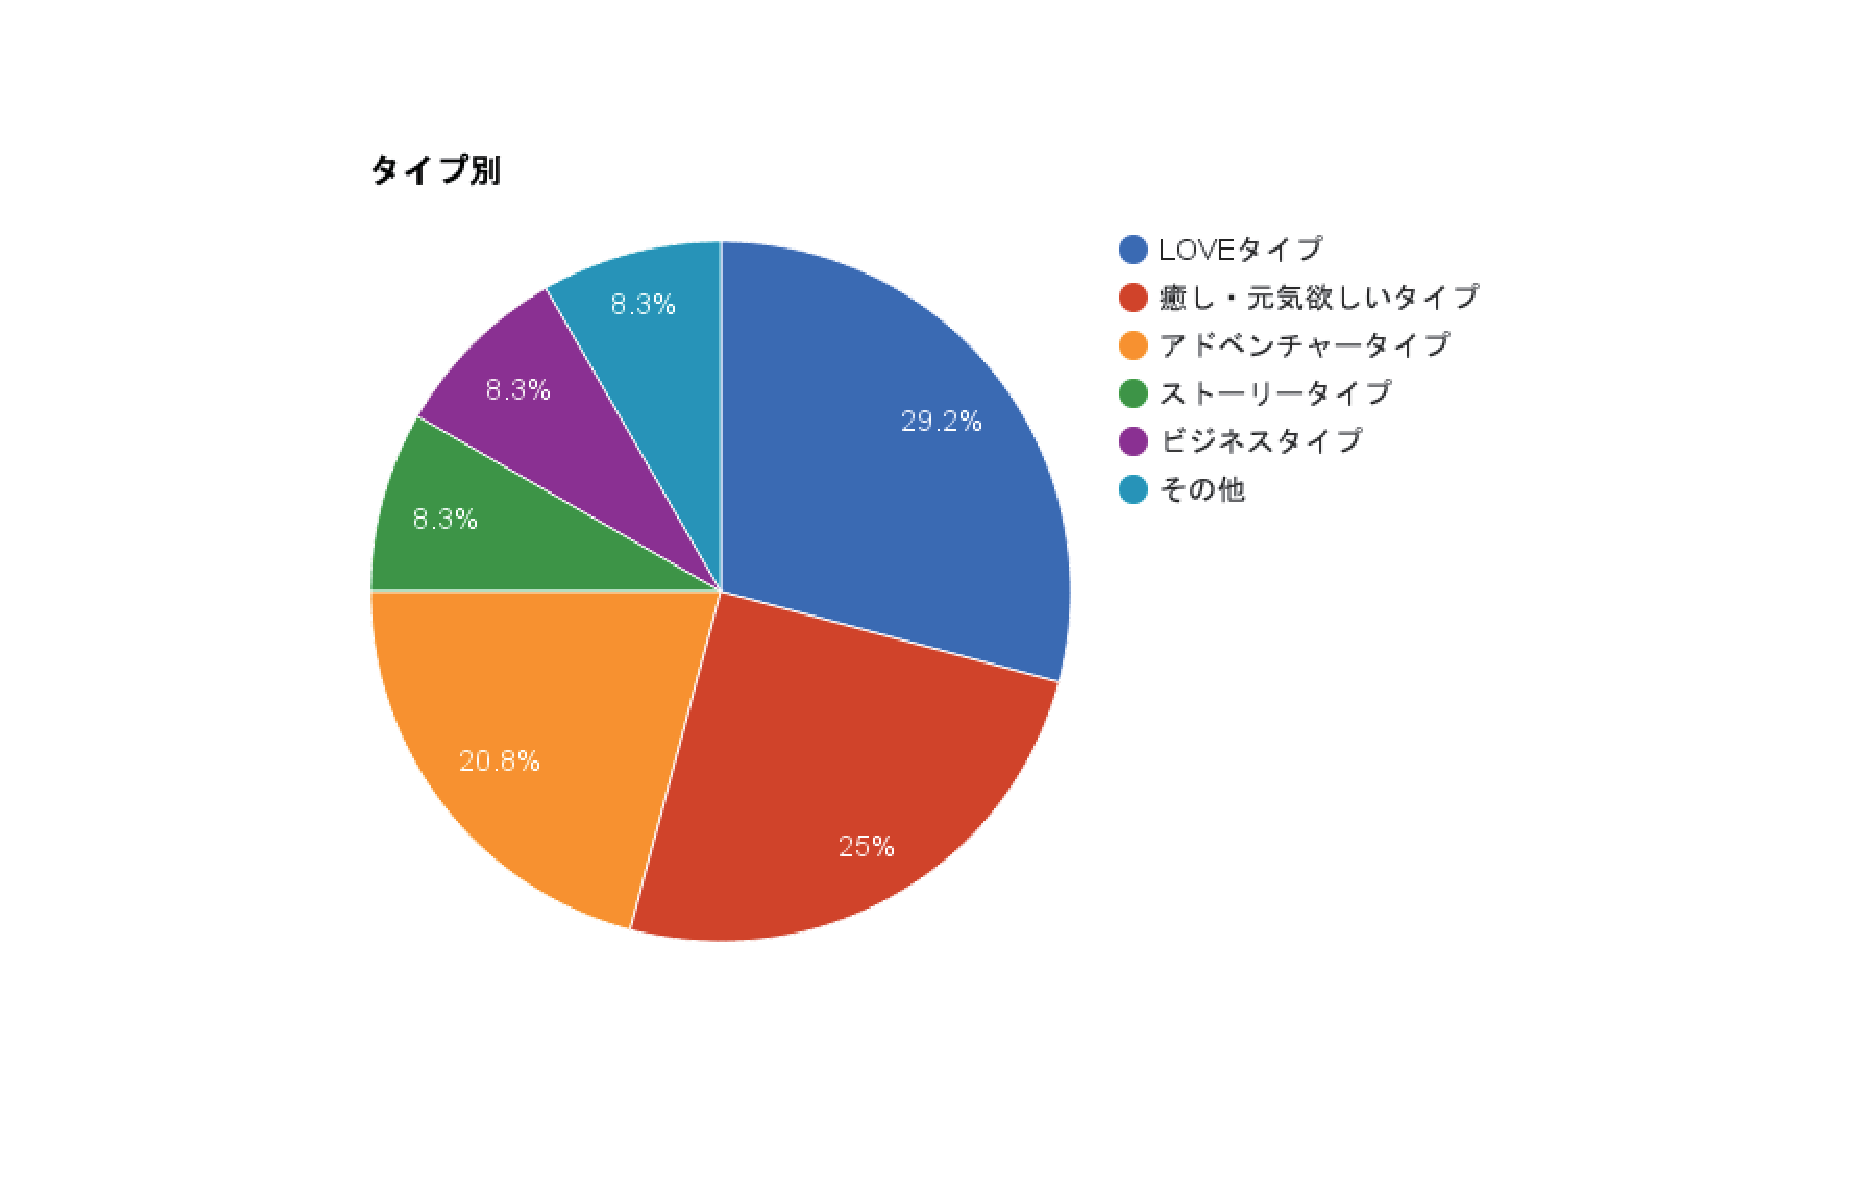
\includegraphics[width=15cm]{eps/dreamType.eps}
\caption{明晰夢で体験したい内容:分析1}
\label{desiredDreamTpye}
\end{center}
\end{figure}

回答をさらに違った方法で分析した結果が\ref{desiredDreamTpye2}である。これらの結果からユーザーによって理想の夢は日常や非日常、具体性や抽象性に隔たりがあり、一貫性が見られないことがわかった。
\begin{figure}[htbp]
\begin{center}
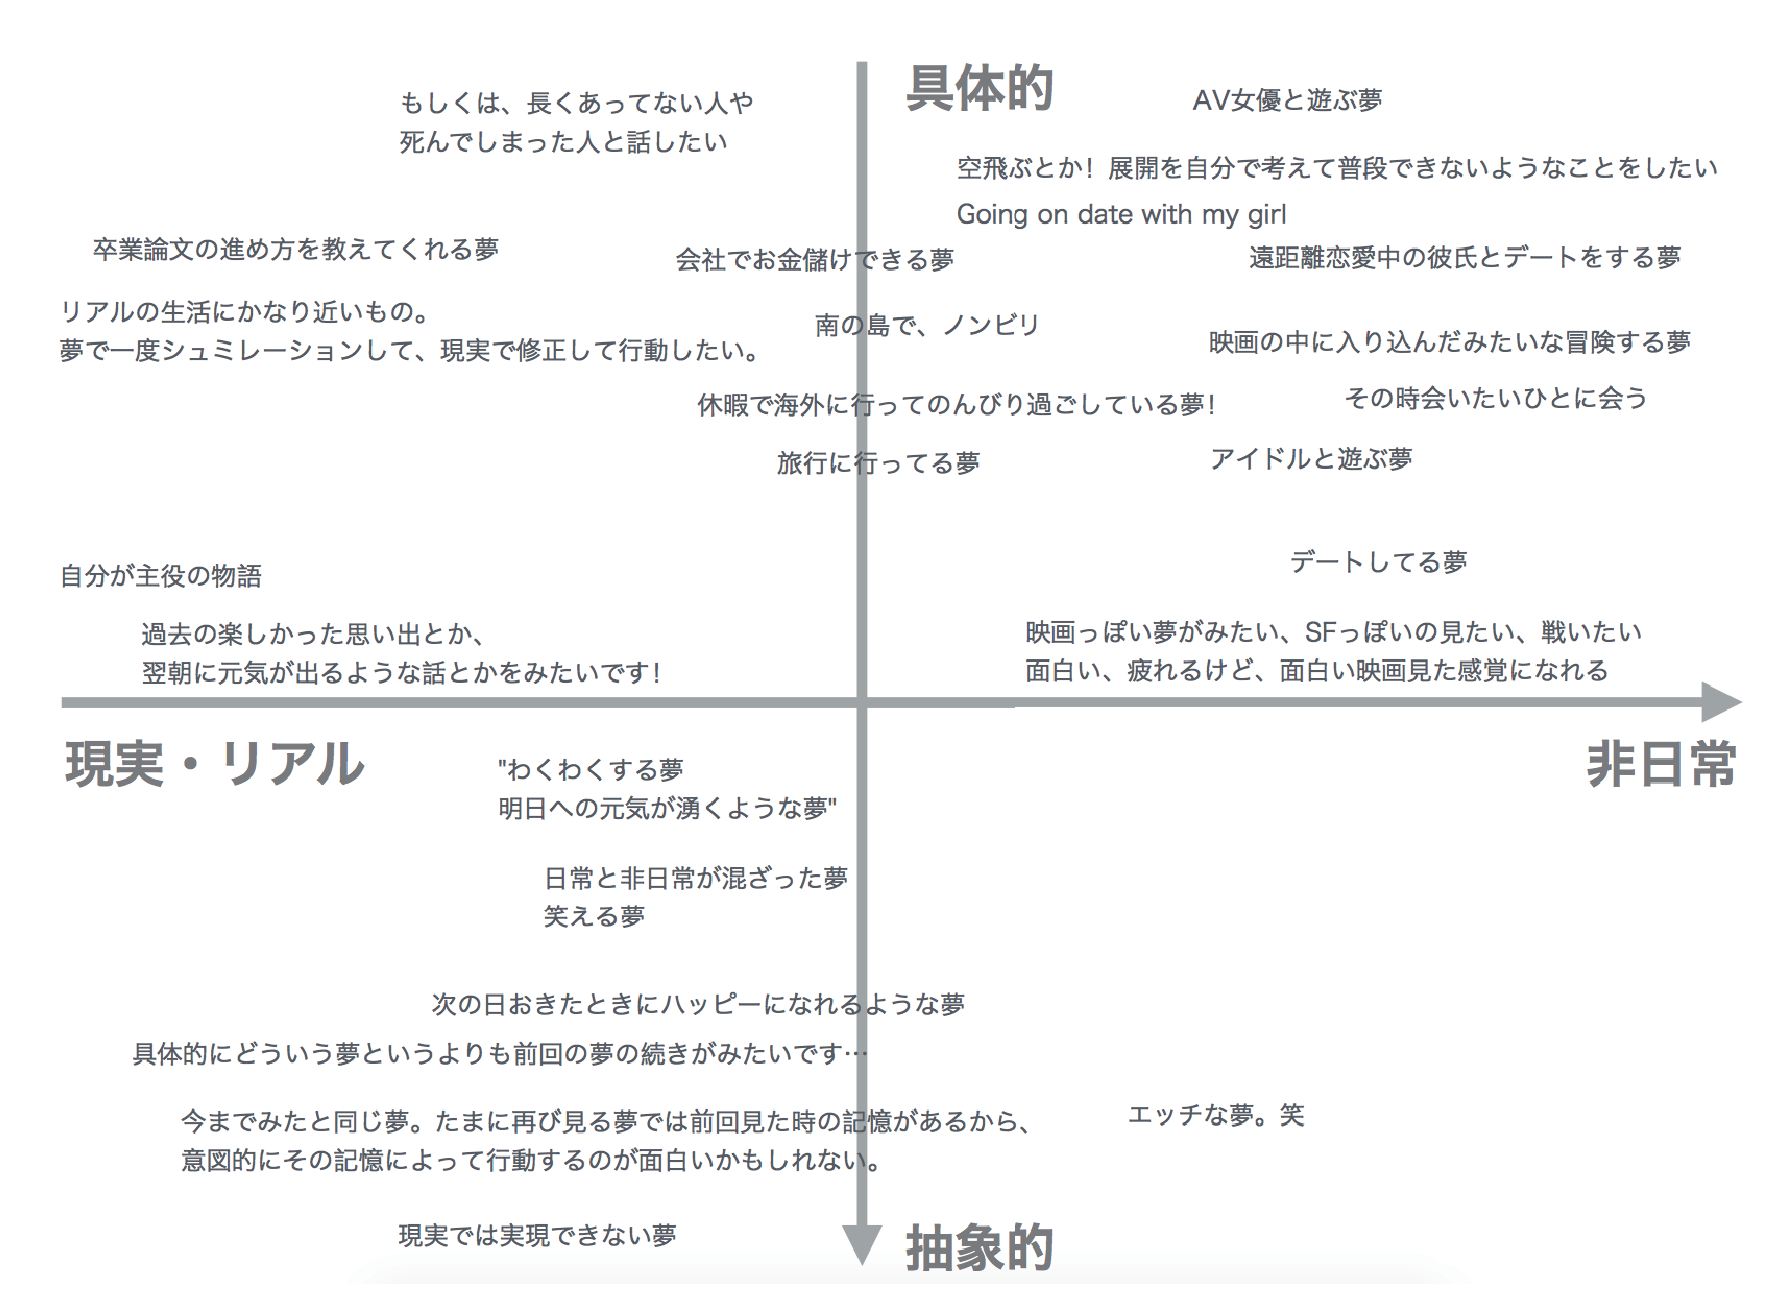
\includegraphics[width=13cm]{eps/whatYouWantToDream.eps}
\caption{明晰夢で体験したい内容:分析2}
\label{desiredDreamTpye2}
\end{center}
\end{figure}

\section{調査から分かったこと}
 オンラインアンケートの結果から現実を仮想的に見ることが明晰夢でも可能なのであれば、DreamTravelerにも興味を示す人が多いということが分かった。明晰夢は睡眠という習慣をより有効に活用し、金銭的コストをかけることなく遂行することができる。求められるのは低価格、高機能、快適なユーザー体験なのでその点に気をつけて開発を進めたい。\\
 夢を操作するにあたって効果が高いと考えられるのは刺激は香りと音でる。そこで、実験を通してどの刺激が最も有効的なのかを調べた。詳細は第4章で述べる。\\
 人は夢を起床後5分以内で忘れてしまうということなので、DreamTravelerにはユーザーが夢の詳細を記入できる夢日記機能を加えることに決めた。夢日記は習慣的につけることで効果が出ると言われている。この事実からDreamTravelerの被験者には2週間前から枕の横に紙とペンを置いて起床後すぐに夢の内容を書く習慣を付けてもらうことにした。\\
 明晰夢で人が見たいと望むコンテンツはには一貫性が無いためDreamTravelerはユーザ一人一人の要望に合った音を選ぶシステムが必要とされることがわかった。DreamTravelerで見ることが可能なコンテンツについては5章で述べる。\\
 Zhang Jieが述べているように夢は記憶の整理のために見るのであれば\cite{Zhang}、記憶と関連性の高い音楽を流す方が効果が出やすいと推測できた。よってDreamTravelerでは様々な音で実験を遂行し、どのような音が夢の操作に適しているのかを検討する。詳細に関しては第6章で述べる。
 
 